%=====================================================================
% MONTAGEM PREDIAL - COMPONENTES REAIS
%=====================================================================
\section{Reconhecimento de componentes reais}

\begin{frame}{Ponto de luz — componentes que aparecem na bancada e na obra}
\begin{columns}[T,onlytextwidth]
\column{0.67\textwidth}
\centering
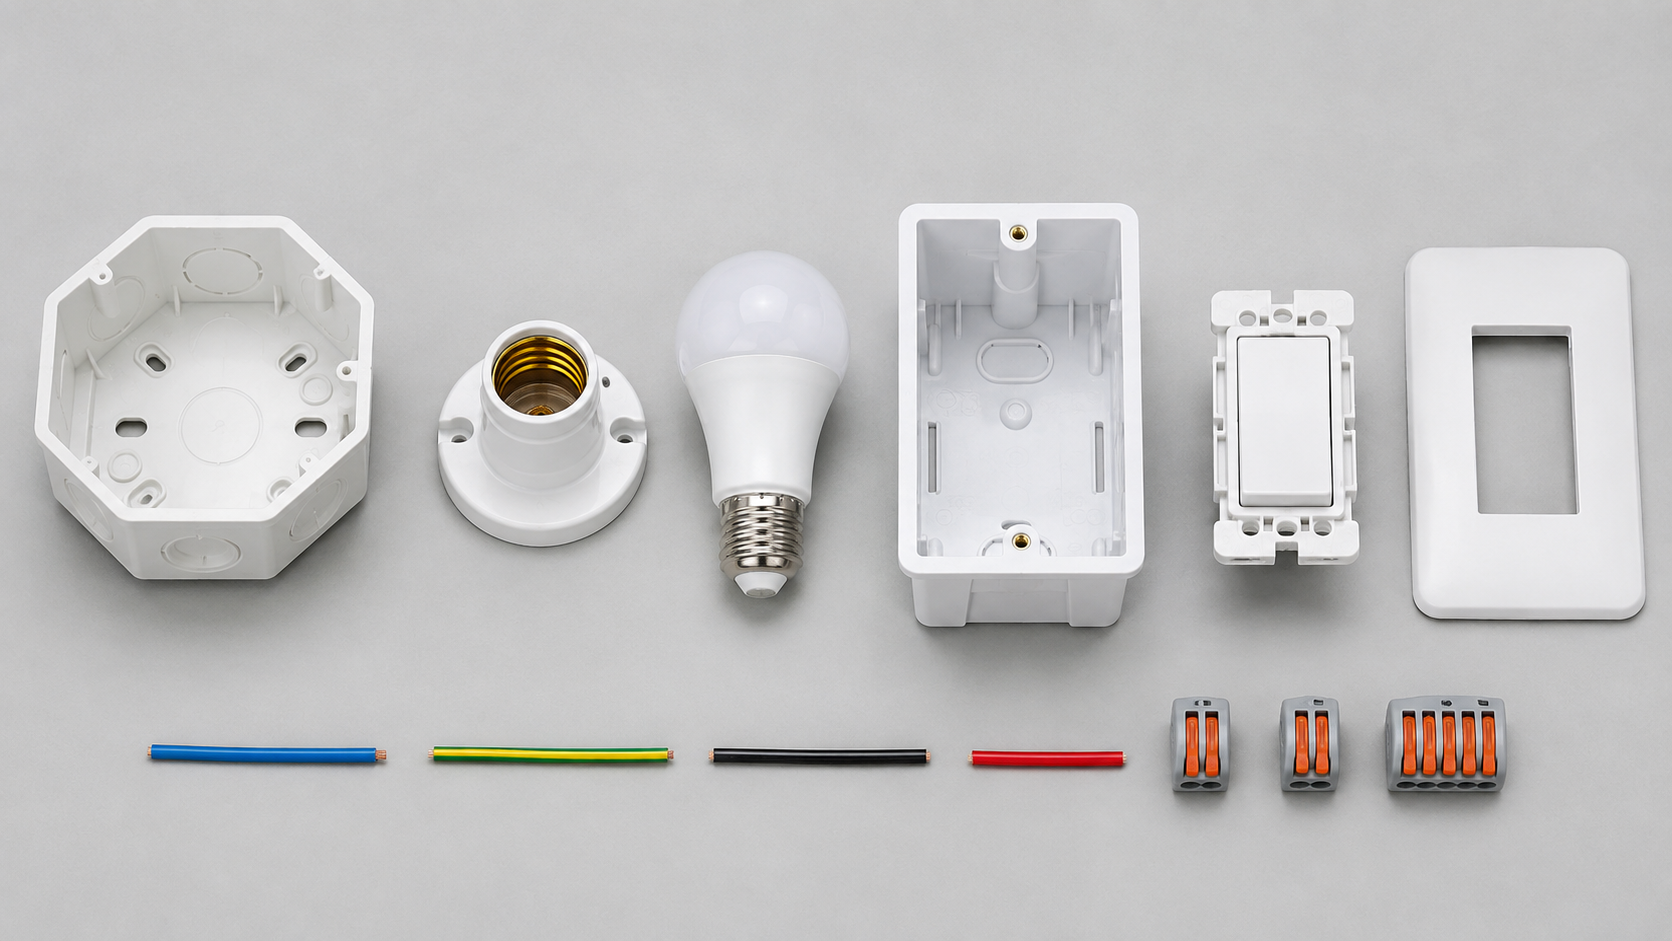
\includegraphics[width=\linewidth,height=.70\textheight,keepaspectratio]{assets/imagens/montagem/componentes_ponto_luz.png}
\column{0.31\textwidth}
\scriptsize
\textbf{Identifique:}
\begin{enumerate}
\item caixa octogonal;
\item soquete/luminária;
\item lâmpada LED;
\item caixa 4$\times$2;
\item interruptor e suporte;
\item placa de acabamento;
\item conectores;
\item condutores por função.
\end{enumerate}
\begin{caixaObs}[title=Regra]
A fotografia reconhece a peça; o esquema define a ligação. A marcação real do borne prevalece sobre a posição aparente.
\end{caixaObs}
\end{columns}
\end{frame}

\begin{frame}{Comandos de iluminação — mecanismos parecidos, funções diferentes}
\begin{columns}[T,onlytextwidth]
\column{0.69\textwidth}
\centering
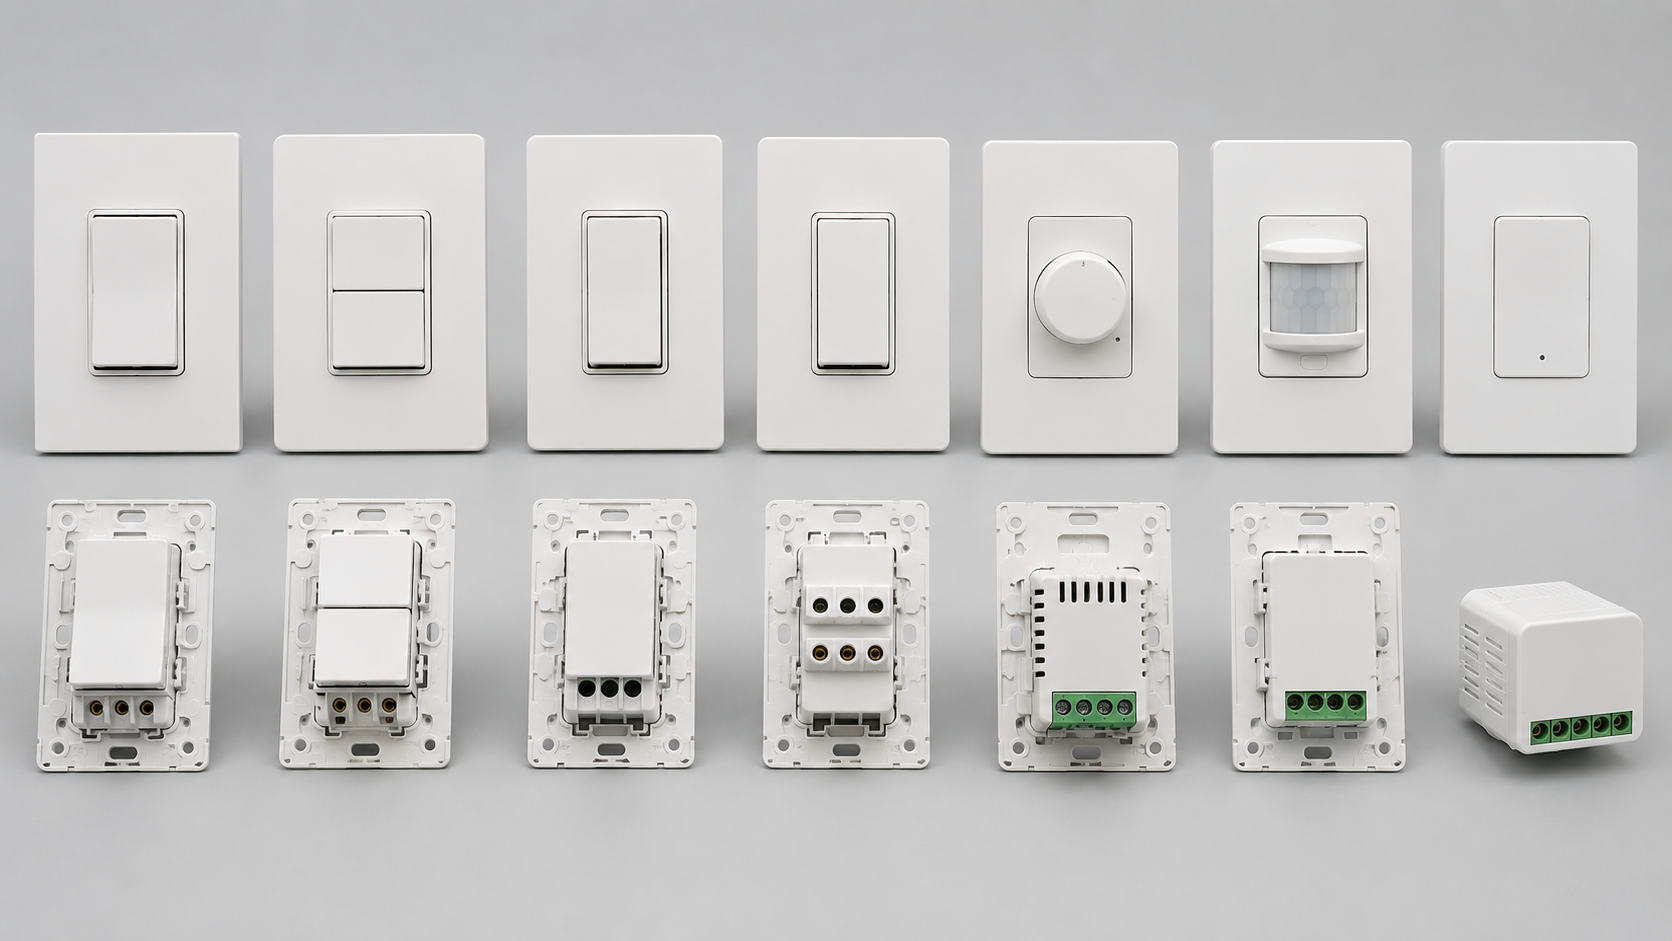
\includegraphics[width=\linewidth,height=.70\textheight,keepaspectratio]{assets/imagens/montagem/componentes_comandos_iluminacao.png}
\column{0.29\textwidth}
\scriptsize
\textbf{Reconheça:}
\begin{itemize}
\item simples;
\item duplo;
\item paralelo;
\item intermediário;
\item dimmer;
\item sensor;
\item comando eletrônico;
\item bornes traseiros.
\end{itemize}
\begin{caixaAt}
Não identificar um mecanismo apenas pela frente. Conferir símbolo, gravação e diagrama do fabricante.
\end{caixaAt}
\end{columns}
\end{frame}

\begin{frame}{Lâmpadas e drivers LED — o conjunto precisa ser compatível}
\begin{columns}[T,onlytextwidth]
\column{0.69\textwidth}
\centering
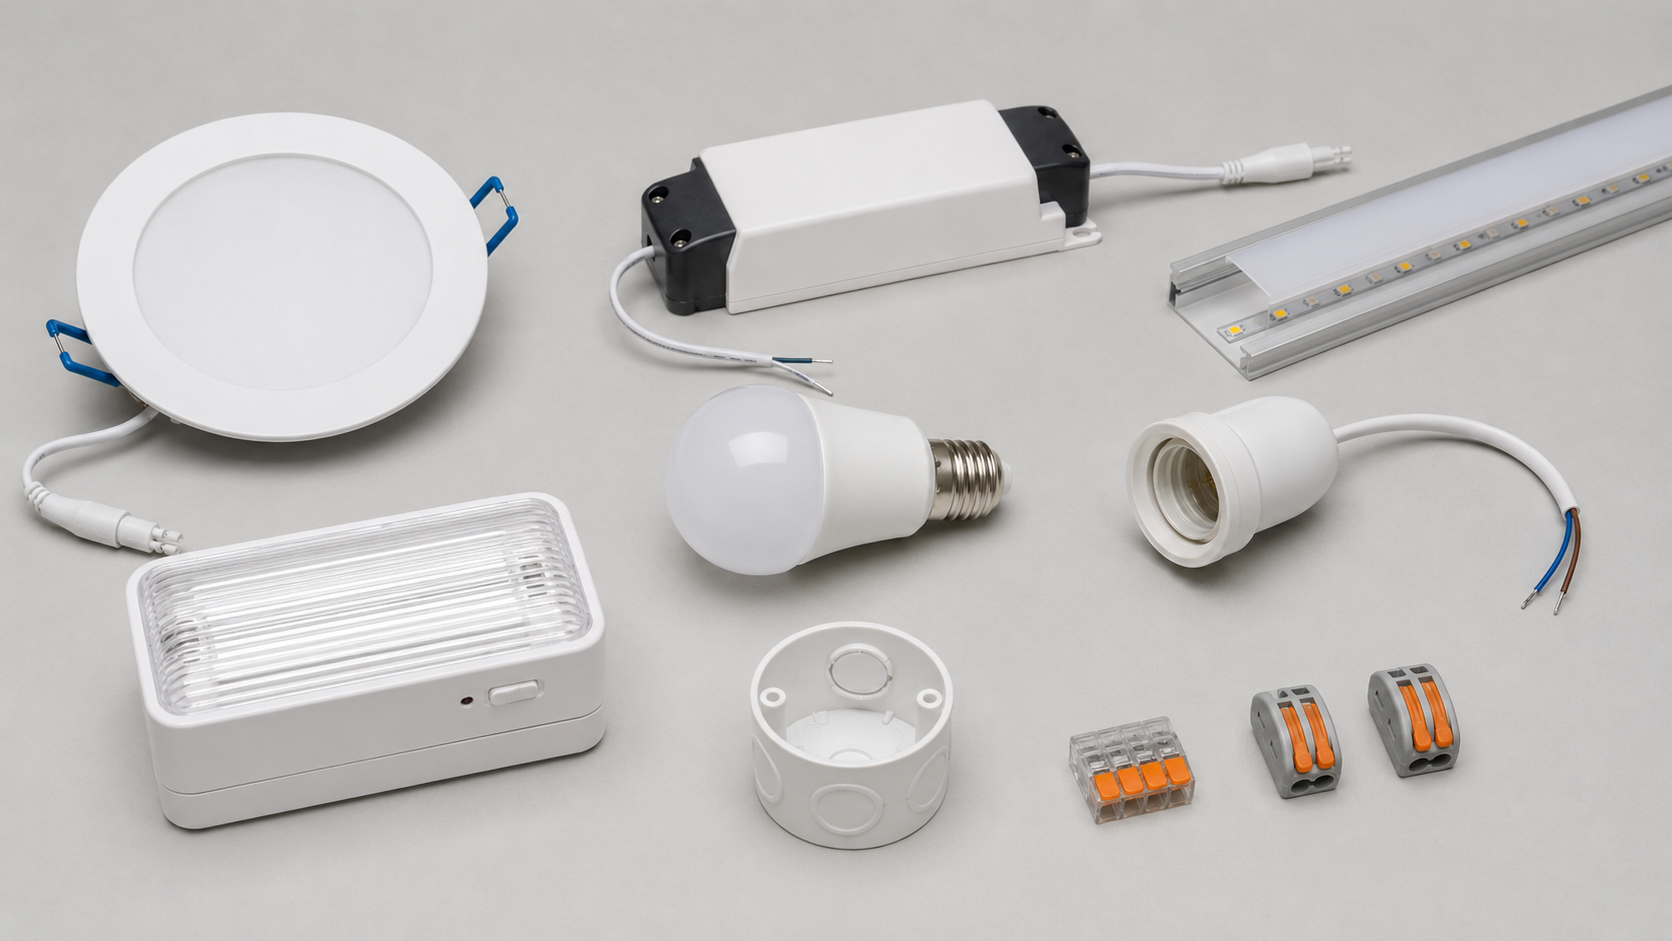
\includegraphics[width=\linewidth,height=.70\textheight,keepaspectratio]{assets/imagens/montagem/componentes_led.png}
\column{0.29\textwidth}
\scriptsize
\textbf{Observe:}
\begin{itemize}
\item lâmpadas com driver integrado;
\item luminárias com driver separado;
\item entradas de rede;
\item saídas de baixa tensão;
\item polaridade quando indicada;
\item potência e corrente nominais;
\item condição de dimerização.
\end{itemize}
\begin{caixaObs}
Driver, dimmer e luminária formam um sistema. Compatibilidade elétrica e de controle deve ser verificada em conjunto.
\end{caixaObs}
\end{columns}
\end{frame}

\begin{frame}{Tomada 2P+T — frente, traseira e bornes}
\begin{columns}[T,onlytextwidth]
\column{0.69\textwidth}
\centering
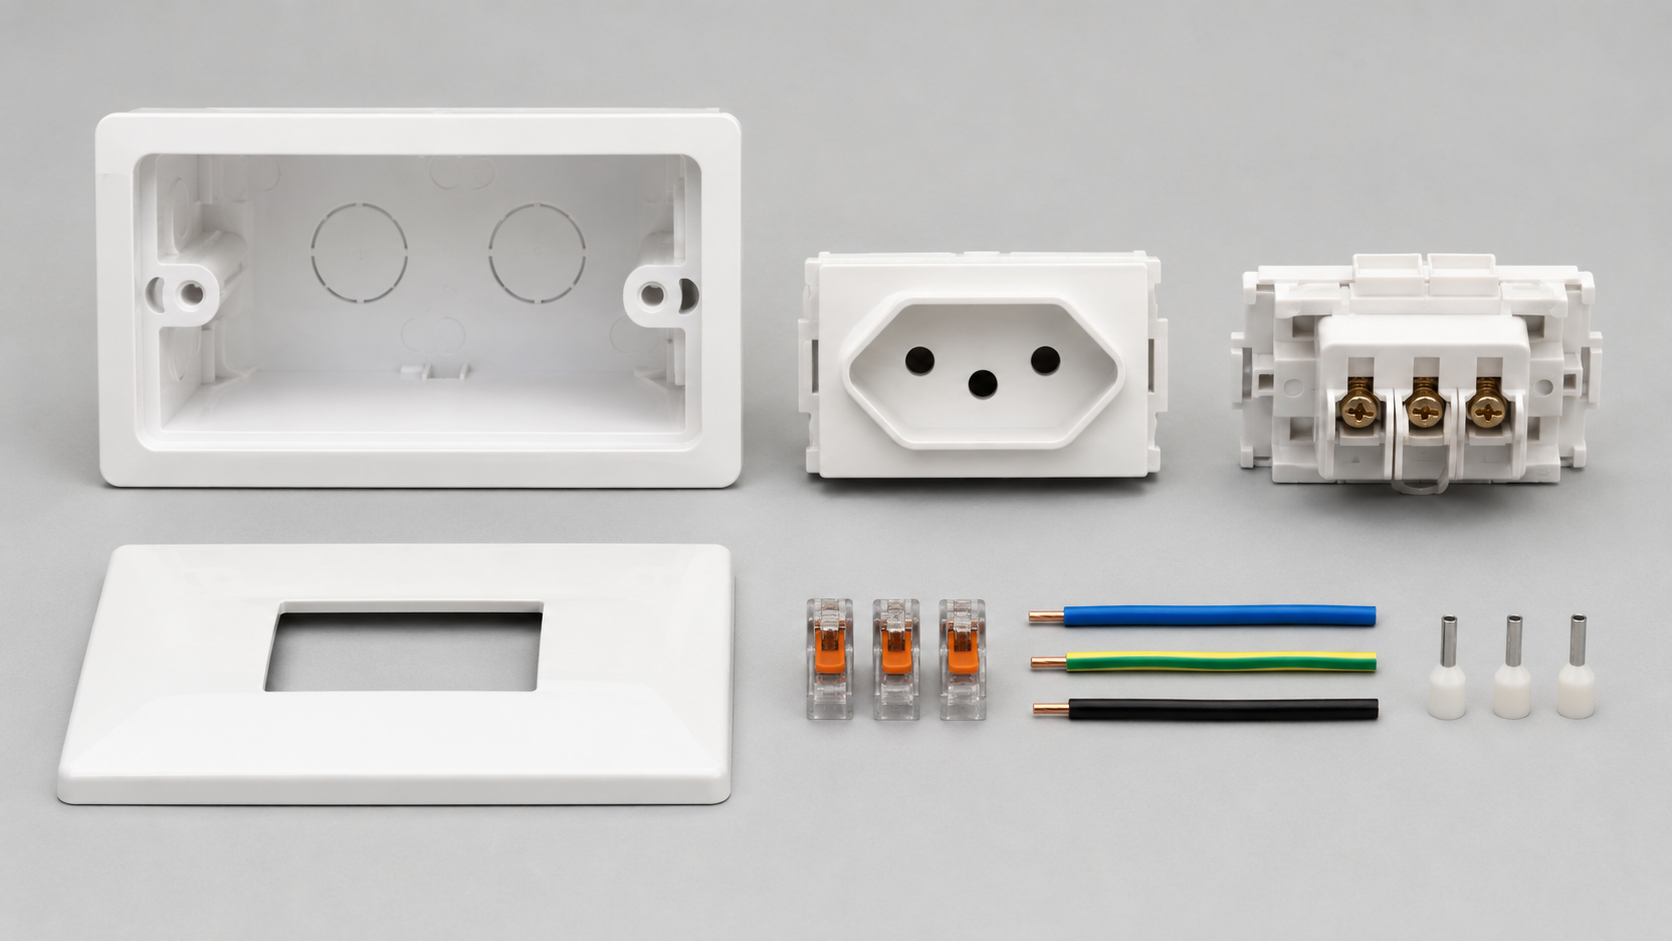
\includegraphics[width=\linewidth,height=.70\textheight,keepaspectratio]{assets/imagens/montagem/componentes_tomada_2pt.png}
\column{0.29\textwidth}
\scriptsize
\textbf{Antes da ligação:}
\begin{itemize}
\item localizar borne de proteção;
\item localizar os dois polos ativos;
\item conferir marcações do fabricante;
\item verificar seção admitida;
\item verificar tipo de conexão;
\item conferir fixação da placa;
\item evitar cobre exposto.
\end{itemize}
\begin{caixaAt}
Vista frontal e vista traseira são opostas. Não deduzir a posição dos bornes olhando apenas a frente do mecanismo.
\end{caixaAt}
\end{columns}
\end{frame}
